% Main-paper figure set (generated by make_figures.py from the sealed n=128 rows).
% Suggested order: Fig.1 is the headline; Figs.1--4 are the quantitative core;
% Fig.5 (behavior) and Fig.6 (6v6 score margin) are optional if space allows.
% Copy the PDFs into figures/ or point \includegraphics at figures_aamas_main/.

% ------------------------------------------------------------------ Fig. 1 (one column)
\begin{figure}[t]
\centering
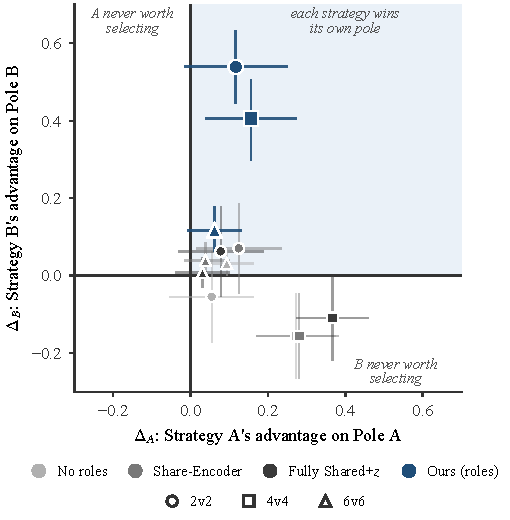
\includegraphics[width=\columnwidth]{figures_aamas_main/fig1_complementarity.pdf}
\caption{Complementary specialization. Each point is one system (color) at one
team size (shape), at its mean $(\Delta_A,\Delta_B)$ over 128 seeds; whiskers are
95\% bootstrap intervals. The shaded upper-right quadrant means each strategy beats
the other on its own opponent, so both are worth selecting. Ours stays in this
quadrant at 2v2, 4v4 and 6v6. At 4v4 every baseline falls into the lower-right
quadrant: its Pole-A strategy also beats its Pole-B strategy on Pole~B.}
\label{fig:complementarity}
\end{figure}

% ------------------------------------------------------------------ Fig. 2 (two column)
\begin{figure*}[t]
\centering
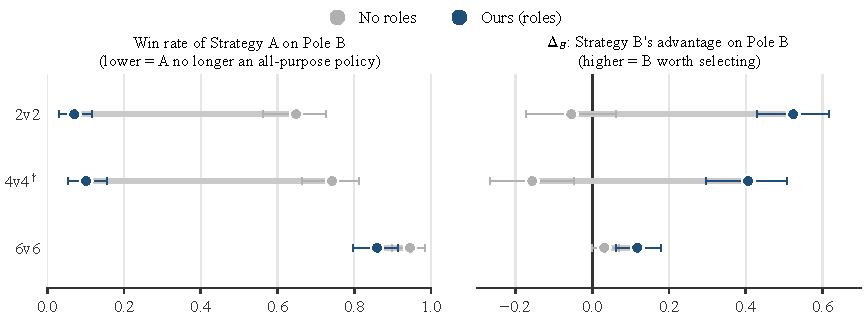
\includegraphics[width=\textwidth]{figures_aamas_main/fig2_mechanism.pdf}
\caption{What roles change. Left: win rate of the Pole-A strategy when it is
deployed on Pole~B. Without roles it is an all-purpose policy (0.65, 0.74, 0.95 at
2v2/4v4/6v6); with roles it drops to 0.07, 0.10 and 0.86. Right: as a result,
$\Delta_B$ moves from $-0.055$, $-0.156$, $+0.031$ to $+0.523$, $+0.406$, $+0.117$,
so the Pole-B strategy becomes worth selecting. Whiskers are 95\% bootstrap intervals
over 128 seeds. 2v2 and 6v6 compare paired seed blocks. $^\dagger$4v4 compares
runs on different seed blocks and is descriptive.}
\label{fig:mechanism}
\end{figure*}

% ------------------------------------------------------------------ Fig. 3 (two column)
\begin{figure*}[t]
\centering
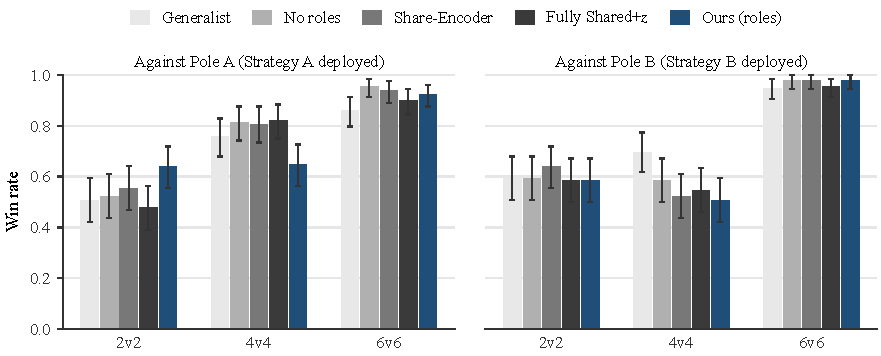
\includegraphics[width=\textwidth]{figures_aamas_main/fig3_deployed_winrate.pdf}
\caption{Raw win rate when each system deploys its intended strategy (Pole-A
strategy on Pole~A, Pole-B strategy on Pole~B; the Generalist uses its single
policy on both). Bars are means over 128 seeds; whiskers are 95\% bootstrap
intervals. Ours is not optimized for raw win rate. At 4v4 the Generalist and the
sharing baselines win more games, but Figure~\ref{fig:complementarity} shows that
their two strategies are not complementary. At 6v6 every system wins 0.86--0.98 of
games.}
\label{fig:deployed_wr}
\end{figure*}

% ------------------------------------------------------------------ Fig. 4 (two column)
\begin{figure*}[t]
\centering
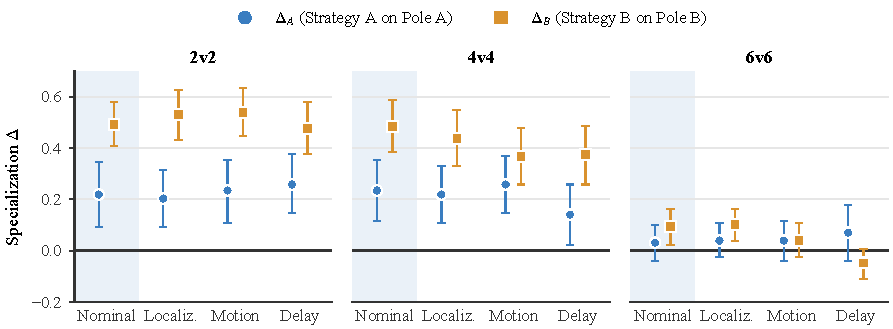
\includegraphics[width=\textwidth]{figures_aamas_main/fig4_robustness.pdf}
\caption{Specialization of our system under medium-severity deployment noise
(localization error, motion noise, observation delay), 128 seeds per condition;
whiskers are 95\% bootstrap intervals. The shaded column is the noise-free
reference. Both mean effects stay positive under every perturbation at 2v2 and
4v4, and under localization and motion noise at 6v6, where the intervals are wider
and some cross zero. At 6v6, observation delay is the
one failure: $\Delta_B$ drops to $-0.047$.}
\label{fig:robustness}
\end{figure*}

% ------------------------------------------------------------------ Fig. 5 (two column, optional)
\begin{figure*}[t]
\centering
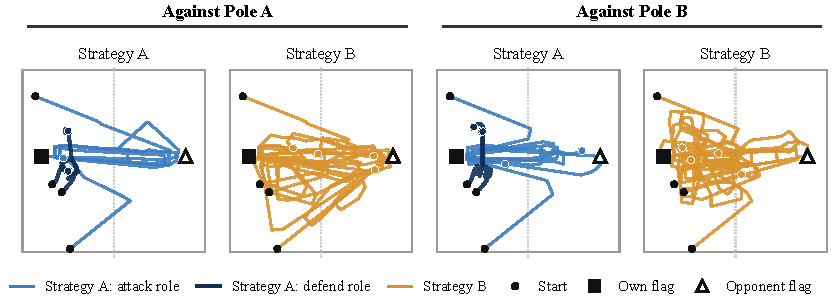
\includegraphics[width=\textwidth]{figures_aamas_main/fig5_trajectories_4v4.pdf}
\caption{Example 4v4 trajectories of our system (one seed, first 80 decision steps)
for the four strategy--opponent pairings. The Pole-A strategy splits its agents into
attackers (light blue), which run at the opponent flag, and defenders (dark blue),
which stay near the own flag. The Pole-B strategy does not split its agents this way.
These trajectories illustrate the behavior only; no quantitative claim rests on them.}
\label{fig:trajectories}
\end{figure*}

% ------------------------------------------------------------------ Fig. 6 (one column, optional)
\begin{figure}[t]
\centering
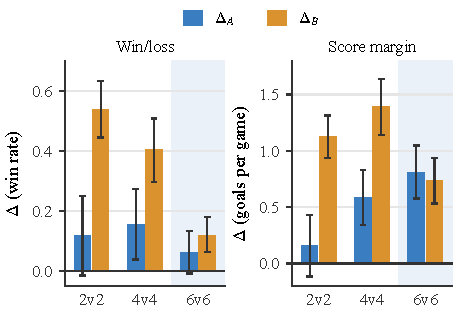
\includegraphics[width=\columnwidth]{figures_aamas_main/fig6_margin.pdf}
\caption{Specialization of our system measured on win/loss (left) and on score
margin, i.e.\ goals scored minus goals conceded (right); 128 seeds, 95\% bootstrap
intervals. At 6v6 (shaded) nearly every game is won, so win/loss differences are
small ($+0.062$, $+0.117$). Score margin is not capped this way, and the two 6v6
strategies separate clearly ($+0.81$ and $+0.73$ goals per game).}
\label{fig:margin}
\end{figure}
